The suggested framework has a total of 8 phases in the classification pipeline which is mentioned in the image presented in table 1.0. The experiments were performed in three scenarios that included pre-training the transfer-learning models on the imageNet, hisbrek dataset and with the random weight initialization in order to evaluate the performance
of each of the models with both partial and complete fine-tuning applied to the target models.

\section{Image Segmention and Preprocessing}
The first phase, targets to obtain the segmented regions of interests from the target source image. 
In order to perform the image segmentation of the source images of 
histopathological images, the pre-processing procedure was performed which involves 
the following sub-procedures which includes color channel separation and 
image normalization and explained in the detailed manner.
\pagebreak
\subsection{Color Channel Seperation}
\begin{figure}[!htp]
    \centering
    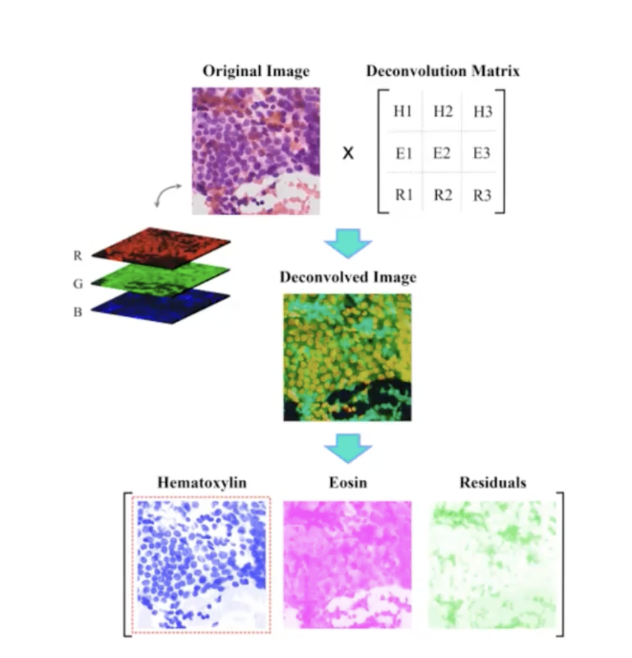
\includegraphics[scale=0.75]{assets/pre-processing.png}
    \caption{Image Credits: MSC Thesis Examination (Presentation) - Mohammad Amin Shamshiri}
    \label{fig:colorchannelseperation}
\end{figure}
Color channel separation as shown in the figure \ref{fig:colorchannelseperation} which aims at decomposing three color channels of the nucleus rather than the other components which are present within the image. In order to perform the color channel separation task, 
the deconvolutional matrix was applied to extract the feature maps of three distinct kinds that involve hematoxylin, Eosin and residuals. Upon investigation, the hematoxylin feature maps were most prominent and were used for the further normalization and segmentation. 


\subsection{Image normalization}
The normalization of the images are performed in order to ensure that the images are easier to process and each pixel in the image is normalized to range within 0 and 1 pixel values rather than 0 and 255, which is easier to train on the convolutional neural networks \citep{rashid_2019}.  

\subsection{Problems with using the UNET segmentation }
In the early phase of the experiments, the semantic segmentation was performed on the hematoxlyin images with the objective of grouping each pixel in the images into the group of nuclei-interior, nuclei-edge, or the background using the famous U-Net model, which requires the manual segmentation of the images and that is a very time-consuming process. The subset of the original dataset was used to evaluate the performance of the segmented images upon splitting the dataset into the training and validation datasets, respectively. However, the quantitative analysis of the U-Net segmentation was not possible and could only be evaluated on a visual basis. Therefore for further investigation, the intensity thresholding technique has been opted to deal with such problems and provide a reliable mechanism for image segmentation.
\subsection{Intensity Thresholding Segmention}

The simple and non-contextual technique focuses on segmenting the images based on the pixel values' replacement with zero in case the corresponding pixel value is less than threshold or 255 otherwise \citep{lectureimagesegmentation}. 
The result of the segmentation is the binary map of the isolated cell nuclei from other components of the image.

\begin{figure}[!htp]
    \centering
    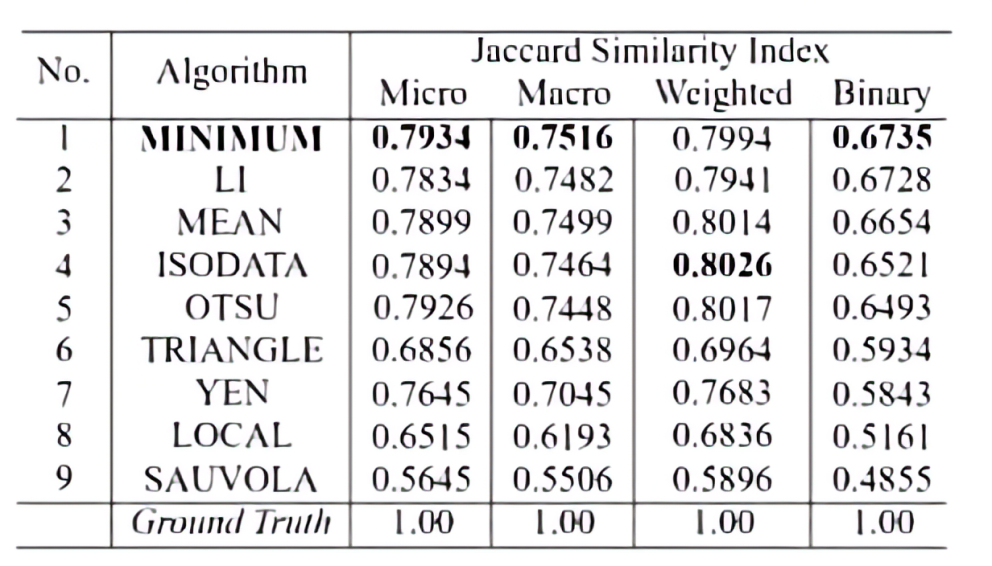
\includegraphics[scale=0.2]{assets/JaccardSimilarity.png}
    \caption{Image Threshold Segmentation}
    \label{fig:jaccardmetrics}
\end{figure} 

 
During the investigation, nine respective algorithms available in the scikit-learn framework as mentioned in the table  \ref{fig:jaccardmetrics} were evaluated. 
The quantitative analysis of the jacquard index has been opted to compare the performance of various available algorithms which is the ratio of size of the intersection between two sets to size of union of two sets. 
Upon investigation it was found that the minimum algorithm as mentioned in the table out performs all the other algorithms and therefore, has been selected for the segmentation.

\subsection{Building Dataset}

The dataset prepreate phase has been performed in two separate phases, that includes building the data for the pre-training phase and another targets the dataset acquisition for the fine-tuning phase. The process of the data acquisition involved collection of 550 ROI related of 50 among which around 225 were bening and 225 belongs to the malignant category. 

\paragraph*{Pre-training phase}
During the pre-training phase, the histopathological BrekHis dataset was consumed, which has 8 sub-categories collected from the 82 patients. However, to scope and select the domain compatible microscopic images for the pre-training phase only the fibroadenoma and lobular carcinoma were selected as they possess most similar traits to the cytological images. 

\paragraph*{Fine-tuning phase}
In order to prepare the dataset for the fine-tuning phase, the data was collected from the 50 different patients, from each of the patients around 11 samples were collected of cytological images. Furthermore, the cytological data samples were divided into the training, validation and testing phase with samples from  30, 10, 10 patients respectively to train the models.
